\section{Notre solution : la clé USB}
\begin{frame}
\tableofcontents[currentsection]
\end{frame}

\begin{frame}
  \frametitle{Les Outils}
  \begin{columns}[t]
    \begin{column}{10cm}
      \begin{exampleblock}{Les outils proposés}
	\begin{itemize}
	\item VLC Media Player : un lecteur de média.
	\item Audacity : un éditeur audio.
	\item Metronomix : un métronome.
        \item MuseScore : un éditeur de partition.
	\end{itemize}
      \end{exampleblock} 
    \end{column}
  \end{columns}
  \begin{figure}[!h]
    \centering
    
\includegraphics[height = 0.5\textheight]{../images/tool_vlc.png}
    \label{VLC} 
    \caption{VLC}
  \end{figure}
\end{frame}

\begin{frame}
  \frametitle{Le Quizz}
  Le Quizz est composé de 2 écrans :
  \begin{columns}[t]
    \begin{column}{10cm}
      \begin{exampleblock}{L'écran de quizz}
	\begin{itemize}
        \item Question au format texte, image ou son.
        \item Réponse à choix multiples.
        \item Explication du professeur.
        \item Temps limité.
        \end{itemize}
      \end{exampleblock} 
    \end{column}
  \end{columns}  
\end{frame}

\begin{frame}
  \frametitle{Le Jeu}
  Le jeu s'inspire du classique \textbf{Space Invaders}.
  \begin{itemize}
    \item Le joueur contrôle un vaisseau qui doit attaquer des notes de musiques.
    \item La note à attaquer change régulièrement.
    \item La difficulté augmente en fonction du cursus musical des élèves.  
  \end{itemize}

  \begin{figure}[!h]
    \centering
    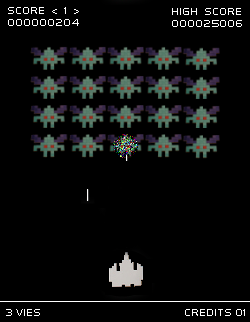
\includegraphics[height = 0.5\textheight]{img/Space_Invaders.png}
    \label{Space Invaders} 
    \caption{Space Invaders}
  \end{figure}
\end{frame}

\begin{frame}
  \frametitle{Administration et aide}
 \begin{columns}[t]
    \begin{column}{10cm}
      \begin{exampleblock}{Les différents menus}
	\begin{itemize}
        \item Un menu qui permet de modifier les données du quizz ou du jeu.
        \item Changer la langue.
        \item Aide pour l'utilisateur.
        \end{itemize}
      \end{exampleblock} 
    \end{column}
  \end{columns}  
\end{frame}
